\subsection{环面上的完整纵横与调和分解}

Hodge 分解在环面上可逐个 Fourier 模态复算，也能直接看见拓扑零模。

球面矢量谐波的 $E/B$ 两类结构有两个不同来源：本征值标签 $\ell,m$ 依赖 $SO(3)$ 作用，恰当与余恰当分解则只依赖微分形式的外微分 $\dd$、Hodge 星 $*$ 与内积。因此，当全局旋转群消失时，后一部分依然可以成立。平直二维环面提供了足够一般、同时又能把每一步 Fourier 计算做到底的检验。

取 $T^2=\RR^2/(2\pi\ZZ)^2$，坐标 $x,y$ 周期为 $2\pi$，度规 $\dd s^2=\dd x^2+\dd y^2$，取正定 Hodge 拉普拉斯算子$\Delta_H=\dd\delta+\delta\dd$。一形式写成 $\alpha=u_x\dd x+u_y\dd y$，取定向 $\dd x\wedge\dd y>0$，则
\begin{equation}\label{eq:ghs-r9-torus-star}
 *(\dd x)=\dd y,\qquad *(\dd y)=-\dd x,
 \qquad *^2=-1\quad\text{（作用于一形式）}.
\end{equation}
周期边界保证分部积分没有边界项，于是 Fourier 模式
\[
 e_k(x,y)=\frac1{2\pi}\ee^{\ii(k_xx+k_yy)},\qquad
 k=(k_x,k_y)\in\ZZ^2
\]
在 $L^2(T^2)$ 中正交归一，并满足 $\Delta_He_k=|k|^2e_k$。非零 $k$ 所对应的任意一形式 Fourier 系数，都是二维复向量。它可以沿 $k$ 和垂直于 $k$ 的方向分别投影。

\begin{theorem}[平直二维环面的一形式 Hodge 分解]
\label{thm:ghs-r9-torus-hodge}
对任意 $L^2$ 一形式 $\alpha$，有正交分解
\begin{equation}\label{eq:ghs-r9-torus-hodge-decomposition}
 \alpha=\dd f+*\dd g+h,
 \qquad \int_{T^2}f\,\dd\mu=\int_{T^2}g\,\dd\mu=0,
 \quad h=c_x\dd x+c_y\dd y.
\end{equation}
函数 $f,g$ 具有弱一阶导数，$h$ 是调和一形式。三个分量在 $L^2$ 意义下两两正交且唯一，$\dim H^1(T^2;\RR)=2$。对每个 $k\ne0$，以 $k^\perp=(-k_y,k_x)$ 记旋转后的波矢，其 Fourier 系数明确满足
\begin{equation}\label{eq:ghs-r9-torus-fourier-projectors}
 \widehat\alpha(k)=\frac{kk^\mathsf T}{|k|^2}\widehat\alpha(k)
 +\frac{k^\perp(k^\perp)^\mathsf T}{|k|^2}\widehat\alpha(k).
\end{equation}
\end{theorem}
\begin{proof}
令 $\widehat\alpha(k)\in\CC^2$ 是一形式两个系数的 Fourier 向量。因为 $k$ 与 $k^\perp$ 正交、长度均为 $|k|$，故两矩阵分别是到两个正交一维空间的投影，且相加为恒等矩阵。令
\[
 \widehat f(k)=\frac{k\cdot\widehat\alpha(k)}{\ii|k|^2},\qquad
 \widehat g(k)=\frac{k^\perp\cdot\widehat\alpha(k)}{\ii|k|^2}
 \quad(k\ne0),
\]
并令两函数的零模为零。由于 $\widehat{\dd f}(k)=\ii k\widehat f(k)$，$\widehat{*\dd g}(k)=\ii k^\perp\widehat g(k)$，\cref{eq:ghs-r9-torus-fourier-projectors} 逐模证明了分解。又因为 $|k|\ge1$，有 $\sum|k|^2|\widehat f(k)|^2\le\sum|\widehat\alpha(k)|^2$，$g$ 同理，故 $f,g\in H^1$，不是只对有限 Fourier 级数成立。

零模 $\widehat\alpha(0)$ 产生常数一形式 $h$。它既闭合也余闭合；另一方面，若某个 $\dd f+*\dd g+h=0$，对非零 $k$ 分别沿 $k$ 与 $k^\perp$ 投影得 $\widehat f(k)=\widehat g(k)=0$，零均值条件令二者为零，剩余 $h=0$。正交性由 Fourier 模态正交及 $k\cdot k^\perp=0$ 成立，故唯一。
\end{proof}

\begin{figure}[htbp]
\centering% Three Hodge components on the flat torus; squares are fundamental domains.
\begin{tikzfig}[scale=.94]
\foreach \x/\ttl in {0/{Exact $\dd f$},3.45/{Coexact $*\dd g$},6.9/{Harmonic $h$}}{
  \draw[thick] (\x,0) rectangle ++(2.45,2.42);
  \node[lecturelabel] at (\x+1.22,2.77) {\ttl};
  \draw[lecturearrow] (\x+.96,0)--(\x+1.40,0);
  \draw[lecturearrow] (\x+.96,2.42)--(\x+1.40,2.42);
}
% Exact mode: horizontal arrows, changes sign across nodal column.
\foreach \y in {.50,1.20,1.90}{
 \draw[lecturearrow] (.98,\y)--(.40,\y);
 \draw[lecturearrow] (1.54,\y)--(2.10,\y);
}
% Coexact mode: vertical circulating arrows at left and right.
\foreach \y in {.45,1.20,1.95}{
 \draw[lecturearrow] (4.02,\y)--(4.02,\y+.32);
 \draw[lecturearrow] (5.34,\y)--(5.34,\y-.32);
}
% Harmonic mode: constant flow, survives as cohomology zero mode.
\foreach \y in {.50,1.20,1.90}{
 \draw[lecturearrow] (7.29,\y)--(8.90,\y);
}
\node[lecturelabel] at (1.22,-.50) {$\delta\dd f\ne0$};
\node[lecturelabel] at (4.67,-.50) {$\delta(*\dd g)=0$};
\node[lecturelabel] at (8.12,-.50) {$\dd h=\delta h=0$};
\end{tikzfig}

\caption{环面一形式的三类不可混同的自由度：沿波矢的恰当部分、横向的余恰当部分、与坐标无关的调和零模。方形相对边识别为同一点，故第三类场不能在不破坏周期性的前提下表示为单值周期势的梯度。}\label{fig:ghs-r9-torus-hodge-classes}
\end{figure}

例如，在一次 Fourier 模态的精确纵横分解的计算中，
令 $f(x,y)=\sin(2x+y)$，记 $\theta=2x+y$，则
\begin{equation}\label{eq:ghs-r9-torus-hodge-sample}
 \dd f=(2\cos\theta)\dd x+(\cos\theta)\dd y,\qquad
 *\dd f=-(\cos\theta)\dd x+(2\cos\theta)\dd y.
\end{equation}
由坐标微分立即得到
\[
 \delta\dd f=5\sin\theta,\quad
 \delta(*\dd f)=0,\quad
 *(\dd*\dd f)=-5\sin\theta.
\]
因此第一类有非零散度而无旋度，第二类无散度而有旋度；两者的 Hodge Laplace 本征值都是 $5$。它们不是两个不同本征值，而是同一 $|k|^2$ 本征空间中的两个正交极化方向。

\begin{figure}[htbp]
\centering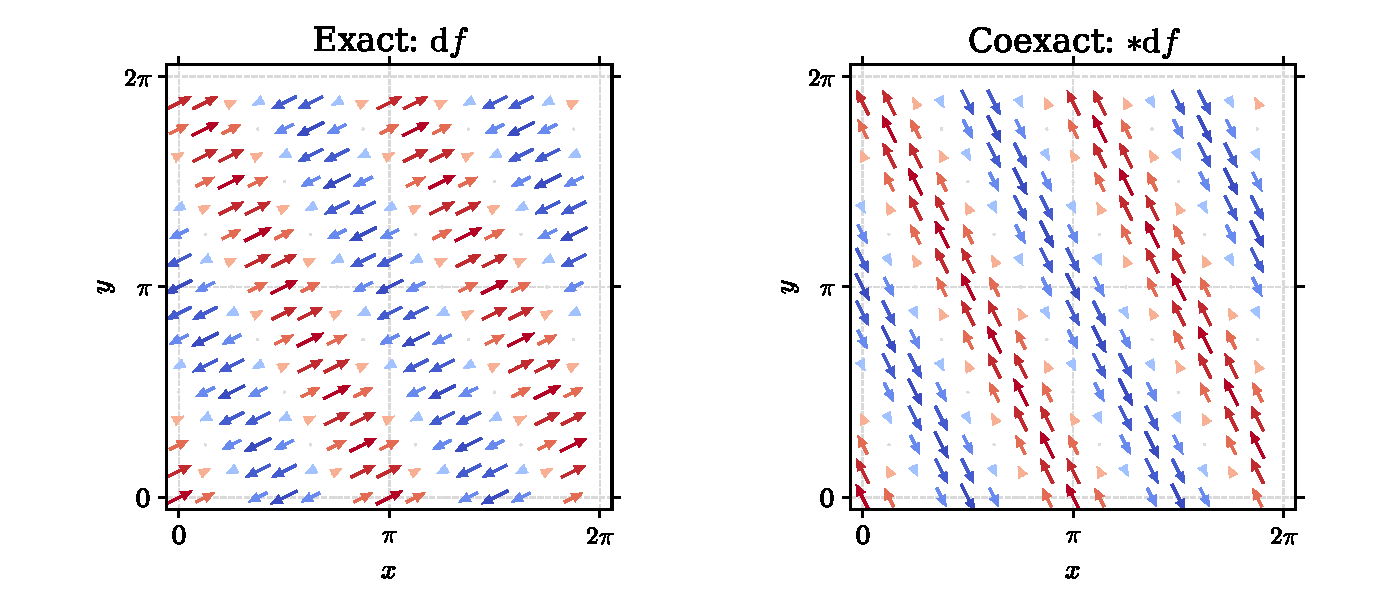
\includegraphics[width=.93\linewidth]{content/MathSkills/figures/geometry-highspin/torus_hodge_vector_modes.pdf}
\caption{\cref{eq:ghs-r9-torus-hodge-sample} 的恰当与余恰当一形式，在环面基本方域上的矢量场箭头。红色表示 $\cos(2x+y)>0$、蓝色表示 $\cos(2x+y)<0$，颜色强度反映其绝对值，两种模式的箭头方向始终正交；边界应按周期识别，不能把图中方域的四条边视为真实物理边界。}\label{fig:ghs-r9-hodge-vector-modes}
\end{figure}

图中的两组箭头采用相同的矢量幅度标尺，箭头长度正比于局部 $|\cos(2x+y)|$，方向和颜色共同标示符号；严格的模态范数仍应使用 $\int_{T^2}|\alpha|^2\dd\mu$。当背景是任意闭定向曲面 $\Sigma$ 时，Hodge 定理仍给出 $\alpha=\dd f+*\dd g+h$，但 $h$ 的维数改为 $2\operatorname{genus}(\Sigma)$，而且不再有简单的整数平面波标签。对有边界的曲面，还必须指定绝对或相对 Hodge 边界条件，才能谈正交分解与零模维数。
